\documentclass[a4paper, 11pt]{article}
\usepackage[spanish]{babel} % Idioma
\usepackage[utf8]{inputenc} % Codificación
\usepackage[T1]{fontenc} % Codificación
\usepackage{amsmath} % Mates
\usepackage[vmargin=2cm,hmargin=2cm]{geometry} % Márgenes
\usepackage{hyperref} % Enlaces
\usepackage{accents} % Cosas de Windows
\usepackage{framed} % Frames

%% Especificaciones de ordenadores
\newcommand{\spec}[6]{
	\bgroup
	\def\arraystretch{1.2}
	\begin{tabular}{|l|}
		\hline
		PC de \textbf{#1} con optimización -O#6\\
		CPU: #2 @#3 GHz\\RAM: #4 GB \hspace{0.8cm} SO: #5 \\
		\hline
	\end{tabular}
	\egroup
	\vspace*{0.2cm}
}

%% Código %%
\usepackage{listings} % Códigos
\usepackage{xcolor} % Colores

\definecolor{backg}{HTML}{F2F2F2}    % Fondo
\definecolor{comments}{HTML}{BDBDBD} % Comentarios
\definecolor{keywords}{HTML}{08388c} % Palabras clave
\definecolor{strings}{HTML}{0489B1}  % Strings

\lstset{
	language=C++,
	basicstyle=\ttfamily,
	breaklines=true,
	backgroundcolor=\color{backg},
	keywordstyle=\color{keywords},
	commentstyle=\color{comments},
	stringstyle=\color{strings},
	tabsize=2,
	% Acentos, ñ, ¿, ¡ (tex.stackexchange.com/questions/24528)
	extendedchars=true,
	literate={á}{{\'a}}1 {é}{{\'e}}1 {í}{{\'i}}1 {ó}{{\'o}}1
	{ú}{{\'u}}1 {ñ}{{\~n}}1 {¡}{{\textexclamdown}}1
	{¿}{{?`}}1
}

% variousconsequences.com/2009/04/maxima-latex-listings.html
\lstdefinelanguage{Maxima}{keywords={find_root},sensitive=true}

%% Imágenes %%
\def\arraystretch{1.2} % Añade padding a todas las tablas
\usepackage{float} % Posicionamiento de figure
\usepackage{graphicx} % Imágenes
\graphicspath{{img/}} % Las imágenes están en la carpeta img

%% Tablas %%
\usepackage{adjustbox} % Tamaño de tablas
\usepackage{pgfplotstable} % Incluir tablas desde .dat
\pgfplotstableset{ % Estilo de todas las tablas
	sci zerofill,
	column type/.add={|}{},
	every last column/.style={column type/.add={}{|}},
	every head row/.style={before row=\hline},
	after row=\hline,
}

\title{\Huge \textbf{Práctica 4}}
\author{\textbf{Pablo Baeyens Fernández} \\ \textbf{Antonio Checa Molina} \\
	\textbf{Iñaki Madinabeitia Cabrera} \\  \textbf{José Manuel Muñoz Fuentes} \\
	\textbf{Darío Sierra Martínez} \\ }
\date{Algorítmica}

\begin{document}
	\maketitle
	\tableofcontents
	\newpage

\section{Estación de ITV}

En este problema se presenta una estación de ITV de $m$ líneas, entre las que
se pretende repartir un grupo de $n$ coches tales que cada coche requiere un
tiempo de inspección $T_i$ (independiente de la línea a la que se haya asignado)
de forma que el tiempo transcurrido desde el inicio hasta que terminen las
inspecciones sea mínimo. Por ello, se buscará organizar los coches en las $m$
líneas buscando que el máximo de la suma de los tiempos de inspección de cada
línea sea mínimo. \\

La implementación de los algoritmos es de la forma:
\begin{description}
	\item[Entrada:] Vector de tiempos de los coches $T$ y número de líneas $m$
	\item[Salida:] Vector que indica en la posición $i$ a qué línea va el coche $i$-ésimo
\end{description}

Proponemos un algoritmo que vaya asignando cada vehículo a cada línea, guarde la solución con el mínimo tiempo que se haya encontrado y vuelva atrás cuando la solución actual no pueda ser mejor que la de menor tiempo encontrada hasta el momento. \\

Para obtener una cota inicial utilizaremos un algoritmo greedy, que se limita a insertar cada coche, por orden de mayor a menor tiempo, en la línea que menos ocupada se encuentre. El orden escogido busca que sea más fácil nivelar las líneas:

\lstinputlisting[firstline=38, lastline=67]{cpps/itv.cpp} % TODO: comprobar que no se mueva el código

El algoritmo vuelta atrás propuesto mantiene un vector de enteros, \texttt{elegidos}, que indica en la posición $i$ a qué línea va el coche $i$. Además tiene un vector de enteros, \texttt{asignados}, que mantiene asignaciones incompletas, en las que solo los primeros elementos tienen líneas asignadas, y un vector de tiempos, \texttt{pesos\_asignados}, que mantiene cuánto tiempo asignado tiene cada línea conforme evoluciona el vector de asignaciones incompleto. Aprovechando que las líneas son iguales, supone que el primer vehículo va a la línea 0.

\lstinputlisting[firstline=69, lastline=83]{cpps/itv.cpp} % TODO: comprobar que no se mueva el código

A continuación se ejecuta un algoritmo recursivo que intenta añadir el último elemento asignado a cada una de las líneas disponibles siempre que esto no provoque que esa línea pase a tener un tiempo asignado mayor que el tiempo máximo de la mejor solución encontrada hasta el momento (que, al inicio de la ejecución del algoritmo, se fija a una solución encontrada por el algoritmo greedy). Además, se evita añadir elementos en una línea si alguna línea anterior se encuentra vacía, dado que las soluciones obtenidas a partir de esa posición serían iguales que las obtenidas colocando ese coche en la anterior salvo permutación de ambas líneas.

\lstinputlisting[firstline=19, lastline=37]{cpps/itv.cpp} % TODO: comprobar que no se mueva el código

Puede observarse que la función de factibilidad consiste en comprobar que la línea donde se piense insertar el coche no tome más peso que el máximo de la mejor solución encontrada, sin comprobar que esto tampoco ocurra en el resto de líneas, pero esto sí se comprueba a la hora de determinar si una solución completa es la mejor solución. Que la función de factibilidad solo compruebe la línea donde se va a insertar se debe a que esta comprobación es mucho más rápida y compensa el mayor número de ramas que se exploran, mientras que es necesario hallar la cota exacta en la solución completa porque la última línea a la que se haya asignado un vehículo podría no ser la que esté más ocupada, y es necesario calcular la cota exacta.

\subsection{Estudio empírico de la eficiencia}

Desde una perspectiva experimental rápidamente vemos que el árbol de posibilidades que tiene que explorar el algoritmo de Backtraking es inmenso; tanto que para más de 20 coches y 10 lineas de el tiempo comienza a volverse un problema inabarcable.

Aquí presentamos una gráfica de varias ejecuciones del algoritmo, que presentamos en escala logarítmica, ya que si no el crecimiento de la función es inapreciable.
\begin{center}
	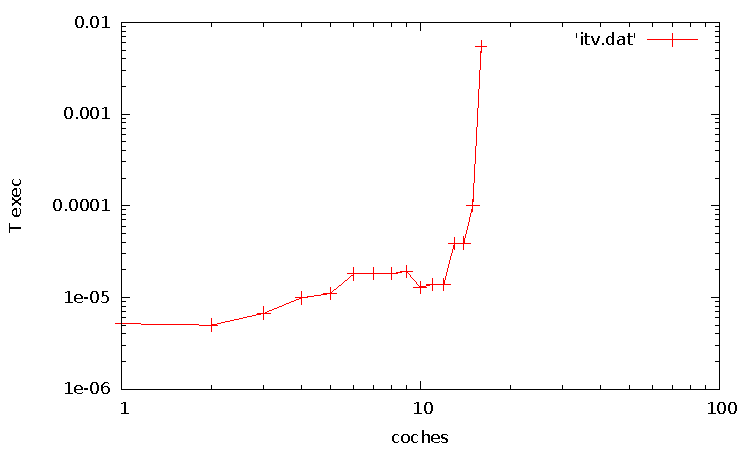
\includegraphics{./img/itvEficiencia}
\end{center}

El crecimiento de la gráfica es desmedido; de hecho las ejecuciones las están hechas con un número bajo de lineas, 10; debido a dicho crecimiento. Esta función claramente mayora a la exponencial.
\newpage
\subsection{Comparación con el Greedy}

Los algoritmos greedy ofrecen la ventaja de la rapidez, pero es verdad que resuelven el problema de manera óptima, aunque este matiz es a veces insustancial e inapreciable; veamos un claro ejemplo:

\begin{center}
	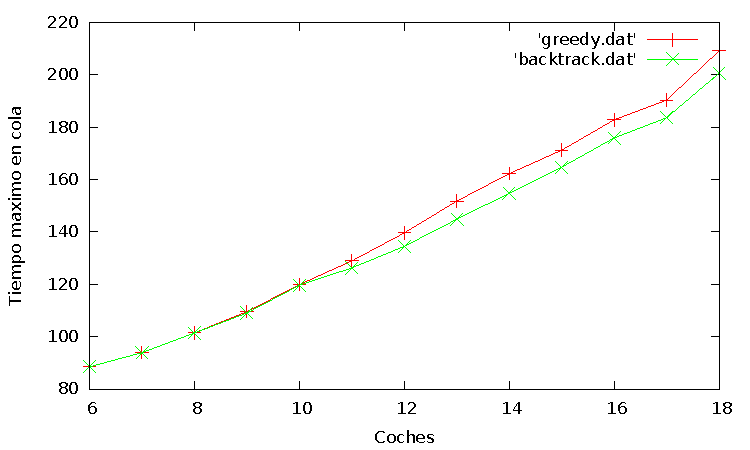
\includegraphics{./img/comp}
\end{center}

Fijamos en esta ejecución el número de colas a 6. Podemos ver como el bactraking es mejor que el greedy, pero la ganancia en prestaciones frente a la perdida en velocidad es nimia. El algoritmo greedy queda, en tiempo, varios ordenes de magnitud por debajo del backtraking a partir de un número relativamente bajo de coches y lineas, en nuestro caso son suficientes 6 lineas y 18 coches para que difieran en 4 ordenes de magnitud.

Volviendo a la ganancia de prestaciones; es incuestionable que mejoramos, pero si el tiempo lo entendemos en segundos la planificación hecha por el greedy tarda varios segundos en completarse más que el bactraking, que en nuestro caso no es relevante.

Como conclusión resaltar lo que hemos ganado frente a lo que hemos perdido, pocas prestaciones frente a mucho tiempo; por tanto a no ser que la solución óptima sea de crucial importancia elegiríamos un greedy en lugar de un bactraking sin dudarlo. Por último como coletazo final cabe mencionar que nuestro algoritmo greedy es con diferencia más fácil de programar.  



% TODO: estudio empírico de la eficiencia

% TODO: comparar con el greedy

% TODO: ¿comparar con fuerza bruta mal enfocada?

\end{document}

>>>>>>> Stashed changes
